\chapter{Режимы двухкластерной синхронизации в полносвязной сети осцилляторов Мэки--Гласса}\label{ch:ch3}

Результаты, полученные в третьей главе, опубликованы в статье \cite{scbib1}. Как и в главе \ref{ch:ch2}, здесь рассматривается полносвязная сеть осцилляторов Мэки--Гласса, в которую добавлен коэффициент связи между элементами сети. В текущей главе решена задача поиска периодических режимов двухкластерной синхронизации --- таких периодических решений, что все компоненты совпадают с одной из двух различных периодических функций.

В разделе \ref{sec:ch3/sect1} описывается система дифференциальных уравнений с запаздывающим аргументом, соответствующая режиму двухкластерной синхронизации. Производится переход к новым переменным. В разделе \ref{sec:ch3/sect2} доказывается обратимость проведённой замены. В разделе \ref{sec:ch3/sect3} для предельной при $\gamma \to +\infty$ системы отыскивается решение, которое при $t \to +\infty$ стремится к периодическому. В разделе \ref{sec:ch3/sect4} доказывается существование периодического режима двухкластерной синхронизации. В разделе \ref{sec:ch3/sect5} приводятся результаты численного моделирования.

%%%%%%%%%%%%%%%%%%%%%%%%%%%%%%%%%%%%%%%%%%%
\section{Постановка задачи}\label{sec:ch3/sect1}
%%%%%%%%%%%%%%%%%%%%%%%%%%%%%%%%%%%%%%%%%%%
Зафиксируем натуральные $m$ и $n$. Рассмотрим полносвязную сеть из $N = m + n$ осцилляторов Мэки-Гласса, т.~е. сеть, в которой каждый осциллятор взаимодействует со всеми остальными. Такая сеть задаётся системой
%
\begin{equation}
	\label{eq:mg_system}
	\dfrac{d V_{j}}{dt}= -bV_{j} + \dfrac{ac\left(V_{j}(t - \tau) + \delta\sum_{k=1,k\neq j}^{N}V_{k}(t)\right)}{1 + \left(c\left(V_{j}(t - \tau) + \delta\sum_{k=1,k\neq j}^{N}V_{k}(t)\right)\right)^{\gamma}}, \quad j=1, 2, \ldots, N,
\end{equation}
где $V_j(t) > 0$ для всех $j = 1, \ldots, N$, коэффициент $\delta > 1$ контролирует силу связи. 

После замен $V_j(t) = c^{-1}u_j(\frac{t}{\tau})$, $\beta = b\tau$, $\alpha=ac\tau$, $t \mapsto \frac{t}{\tau}$,
перейдём от системы (\ref{eq:mg_system}) к более удобной форме с меньшим числом параметров:
%
\begin{equation}
	\label{eq:mg_system_norm}
	\dot{u}_j=-\beta u_j+\frac{\alpha\big(u_j(t - 1) + \delta\sum_{k = 1, k\neq j}^{N}u_{k}(t)\big)}{1+\big(u_j(t - 1) + \delta\sum_{k = 1, k \neq j}^{N}u_{k}(t)\big)^\gamma}, \quad j = 1, 2, \ldots, N.
\end{equation}
%
Здесь $\alpha, \beta > 0$, $u_j(t) > 0$ для всех $j = 1, \ldots, N$.

Пусть
%
\begin{equation}
	\label{eq:F_func}
	F_{\gamma}(x) = \dfrac{x}{1 + x^\gamma}.
\end{equation}

С учётом \eqref{eq:F_func} система \eqref{eq:mg_system_norm} примет вид:
%
\begin{equation}
	\label{eq:mg_system_norm_F}
	\dot{u_j} = -\beta u_j + \alpha\,F_{\gamma}\left(u_j(t - 1) + \delta \sum_{k = 1, k\neq j}^{N}u_{k}(t)\right), \quad j = 1, \ldots, N.
\end{equation}

Будем искать режимы двухкластерной синхронизации, т.~е. периодические режимы, в которых $m$ осцилляторов описываются функцией $u(t)$, а остальные $n$ осцилляторов --- другой функцией $v(t)$.

Система \eqref{eq:mg_system_norm_F} примет вид:
%
\begin{equation}
	\label{eq:mg_cluster_system_norm}
	\begin{cases}
		\dot{u} = -\beta u + \alpha \, F_{\gamma} \big(u(t - 1) + \delta (m - 1) u + \delta n v\big),\\
		\dot{v} = -\beta v + \alpha  \, F_{\gamma} \big(v(t - 1) + \delta m u + \delta (n - 1) v\big).
	\end{cases}
\end{equation}

После замен
\begin{equation}
	\label{eq:tilde_change}
	\tilde{u} = u(t - 1) + \delta (m - 1) u + \delta n v, \quad \tilde{v} = v(t - 1) + \delta m u + \delta (n - 1) v,
\end{equation}
%
система \eqref{eq:mg_cluster_system_norm} примет вид
%
\begin{equation}
	\label{eq:mg_cluster_system_pre_tilde}
	\begin{cases}
		\dot{u} = -\beta u + \alpha \, F_{\gamma}(\tilde{u}),\\
		\dot{v} = -\beta v + \alpha \, F_{\gamma}(\tilde{v}).
	\end{cases}
\end{equation}


Перепишем систему \eqref{eq:mg_cluster_system_pre_tilde} через переменные $\tilde{u}$ и $\tilde{v}$.
\begin{multline*}
	\dot{\tilde{u}} = \dot{u}(t - 1) + \delta (m - 1) \dot{u} + \delta n \dot{v} =\\= \left(-\beta u(t - 1) + \alpha \, F_{\gamma}(\tilde{u}(t - 1))\right) + \delta (m - 1)(-\beta u + \alpha\, F_{\gamma}(\tilde{u})) + \delta n (-\beta v + \alpha \, F_{\gamma}(\tilde{v})) =\\
	= -\beta(u(t - 1) + \delta (m - 1)u + \delta nv) + \alpha\big(F_{\gamma}(\tilde{u}(t - 1)) + \delta (m - 1) \, F_{\gamma}(\tilde{u}) + \delta n \, F_{\gamma}(\tilde{v})\big) = \\
	= -\beta \tilde{u} + \alpha \big(F_{\gamma}(\tilde{u}(t - 1)) + \delta (m - 1)\, F_{\gamma}(\tilde{u}) + \delta n \, F_{\gamma}(\tilde{v})\big).
\end{multline*}

Аналогично,
\[
\dot{\tilde{v}} = -\beta \tilde{v} + \alpha \big(F_{\gamma}(\tilde{v}(t - 1)) + \delta m \, F_{\gamma}(\tilde{u}) + \delta (n - 1) \, F_{\gamma}(\tilde{v})\big).
\]

Получаем систему:
%
\begin{equation}
	\label{eq:mg_cluster_system_tilde}
	\begin{cases}
		\dot{\tilde{u}} = -\beta \tilde{u} + \alpha \big(F_{\gamma}(\tilde{u}(t - 1)) + \delta (m - 1) \, F_{\gamma}(\tilde{u}) + \delta n \, F_{\gamma}(\tilde{v})\big),\\
		\dot{\tilde{v}} = -\beta \tilde{v} + \alpha \big(F_{\gamma}(\tilde{v}(t - 1)) + \delta m \, F_{\gamma}(\tilde{u}) + \delta (n - 1) \, F_{\gamma}(\tilde{v})\big).
	\end{cases}
\end{equation}
% По ходу возник вопрос, почему функции u~ и v~ будут дифференцируемы (в смысле не будет точек, в которых производные справа и слева отличаются, как это бывает в методе шагов). Ответ простой: если в какой-то точке производные бы отличались слева и справа, то правая часть отличалась бы слева и справа, но она непрерывная. Значит, всё ок. Более того, решение непрерывно дифференцируемое, т.к. производные равны непрерывным функциям в правой части.

Поскольку $\tilde{u} > 0$, $\tilde{v} > 0$, можно провести экспоненциальные замены
\begin{equation}
	\label{eq:exp_change}
	\tilde{u} = e^x, \quad \tilde{v} = e^y.
\end{equation}

Вводя новую функцию $G_{\gamma}(x) = e^{-x} \, F_{\gamma}(e^x)$, получаем итоговый вид системы:
\small
\begin{equation}
	\label{eq:system_main}
	\begin{cases}
		\dot{x} = -\beta + \alpha \left(e^{x(t - 1) - x} G_{\gamma}(x(t - 1)) + \delta (m - 1) G_{\gamma}(x) + \delta n e^{y - x} G_{\gamma}(y)\right),\\
		\dot{y} = -\beta + \alpha \left(e^{y(t - 1) - y} G_{\gamma}(y(t - 1)) + \delta m e^{x - y} G_{\gamma}(x) + \delta (n - 1) G_{\gamma}(y)\right).
	\end{cases}
\end{equation}
\normalsize

\section{Обратимость замены}\label{sec:ch3/sect2}

Докажем, что решение $(u, v)$ системы \eqref{eq:mg_cluster_system_norm} однозначно восстанавливается по решению $(x, y)$ системы \eqref{eq:system_main}.

% Здесь нужна дифференцируемость, а не только непрерывность, т.к. дальше в операторе A у нас присутствует производная функции u. Но просто дифференцируемости недостаточно, т.к. пространство дифф. функций не полно, поэтому потребуем непрерывную дифференцируемость. u~, v~ непрерывно дифференцируемы (см. замечание выше), так что всё корректно.
\begin{lemma}
	\label{lm:uv_from_tilde}
	Пусть $\tilde{u}(t), \tilde{v}(t)$ --- $T$-периодические ($T > 0$) непрерывно дифференцируемые функции. Тогда существуют и определены единственным образом непрерывно дифференцируемые $T$-периодические функции $u(t), v(t)$, удовлетворяющие соотношениям \eqref{eq:tilde_change}.
\end{lemma}
\begin{proof}
	Перепишем систему \eqref{eq:tilde_change} в матричной форме:
	\[
	\begin{pmatrix}
		\tilde{u}\\
		\tilde{v}
	\end{pmatrix} = 
	\begin{pmatrix}
		u(t - 1)\\
		v(t - 1)
	\end{pmatrix} +
	\delta \cdot
	\begin{pmatrix}
		m - 1 & n \\
		m & n - 1
	\end{pmatrix}
	\begin{pmatrix}
		u\\
		v
	\end{pmatrix}.
	\]
	
	Обозначим
	\[
	J = 
	\delta \cdot
	\begin{pmatrix}
		m - 1 & n \\
		m & n - 1
	\end{pmatrix}, \quad
	\varphi =
	\begin{pmatrix}
		u\\
		v
	\end{pmatrix}, \quad
	\tilde{\varphi} =
	\begin{pmatrix}
		\tilde{u}\\
		\tilde{v}
	\end{pmatrix}
	\]
	
	Получаем равенство $\tilde{\phi} = \phi(t - 1) + J \phi$. Выразим $\phi$:
	\begin{equation}
		\label{eq:tilde_matrix_form}
		\varphi = 
		J^{-1}
		\left(
		\tilde{\varphi} -
		\varphi(t - 1)
		\right),
		\text{ где }
		J^{-1} = \dfrac{1}{\delta(m + n - 1)} 
		\begin{pmatrix}
			1 - n & n \\
			m & 1 - m
		\end{pmatrix}.
	\end{equation}
	
	Пусть $(C^1[0, T])^2$ --- пространство пар непрерывно дифференцируемых $T$-периодических функций $\mathbb{R} \to \mathbb{R}$ с нормой
	%
	\[\Vert (f, g) \Vert = \Vert f \Vert_{C^1} + \Vert g \Vert_{C^1} = \sup\limits_{[0, T]} |f| + \sup\limits_{[0, T]} |f'| + \sup\limits_{[0, T]} |g| + \sup\limits_{[0, T]} |g'|.\]
	
	Определим оператор $\mathcal{L}:(C^1[0, T])^2 \to (C^1[0, T])^2$:
	%\[\mathcal{L}: \varphi \mapsto \left(\psi: t \mapsto J^{-1} \left[ \tilde{\varphi} - \varphi(t - 1) \right] \right)\]
	\[\mathcal{L}\varphi = J^{-1} \left(\tilde{\varphi} - \varphi(t - 1) \right).\]
	
	Оператор $\mathcal{L}$ является сжимающим на $(C^1[0, T])^2$, т.к.
	\[\Vert\mathcal{L}\varphi - \mathcal{L}\psi\Vert = \Vert J^{-1} (\psi(t - 1) - \phi(t - 1)) \Vert \leq \Vert J^{-1} \Vert \cdot \Vert \psi - \phi \Vert = \dfrac{1}{\delta} \Vert \psi - \phi \Vert,\]
	%
	где $\Vert J^{-1} \Vert = \frac{1}{\delta} < 1$ --- 1-норма матрицы $J^{-1}$.
	
	Поскольку пространство $(C^1[0, T])^2$ полно, существует единственная неподвижная точка $\varphi_*$ оператора $\mathcal{L}$, которая удовлетворяет равенству \eqref{eq:tilde_matrix_form}.
\end{proof}

\begin{lemma}
	\label{lm:uv_inverse_system}
	Пусть $\tilde{u}, \tilde{v}$ --- $T$-периодические функции, являющиеся решением системы \eqref{eq:mg_cluster_system_tilde}. Тогда $T$-периодические функции $u, v$, однозначно выражаемые из соотношений \eqref{eq:tilde_change}, являются решением системы \eqref{eq:mg_cluster_system_norm}.
\end{lemma}
\begin{proof}
	Введём обозначение:
	\begin{equation}
		\label{eq:operator_A_definition}
		A_{m, n}(u, v) = -\beta u + \alpha \, F_{\gamma}\big(u(t - 1) + \delta (m - 1)u + \delta n v \big) - \dot{u}.
	\end{equation}
	%
	Тогда система \eqref{eq:mg_cluster_system_norm} при фиксированных $m, n$ примет вид
	\begin{equation}
		\label{eq:uv_system_operator_form}
		\begin{cases}
			A_{m, n}(u, v) = 0,\\
			A_{n, m}(v, u) = 0.\\
		\end{cases} 
	\end{equation}
	%
	Пусть $\tilde{u}, \tilde{v}$ --- $T$-периодическое решение системы \eqref{eq:mg_cluster_system_tilde}. Поскольку правая часть системы \eqref{eq:mg_cluster_system_tilde} непрерывна, функции $\tilde{u}, \tilde{v}$ непрерывно дифференцируемы. По лемме \ref{lm:uv_from_tilde}, функции $u, v$, однозначно выражаемые из соотношений \eqref{eq:tilde_change}, также будут $T$-периодичны и непрерывно дифференцируемы. Докажем, что они удовлетворяют системе \eqref{eq:uv_system_operator_form}.
	
	Из определения \eqref{eq:operator_A_definition} следуют равенства
	\[
	\begin{cases}
		\dot{u}(t - 1) + A_{m, n}(u(t - 1), v(t - 1))  = -\beta u(t - 1) + \alpha \, F_{\gamma}(\tilde{u}(t - 1)),\\
		\delta (m - 1)\dot{u} + \delta (m - 1) A_{m, n}(u, v)  = -\delta \beta (m - 1) u + \delta \alpha (m - 1) \, F_{\gamma}(\tilde{u}),\\
		\delta n \dot{v} + \delta n A_{n, m}(v, u)  = -\delta \beta n v + \delta \alpha n \, F_{\gamma}(\tilde{v}).
	\end{cases}
	\]
	%
	Складывая их, получаем
	\small
	\begin{multline*}   
		(\dot{u}(t - 1) + \delta (m - 1)\dot{u} + \delta n\dot{v}) + A_{m, n}(u(t - 1), v(t - 1)) + \delta (m - 1) A_{m, n}(u, v) + \delta n A_{n, m}(v, u) =\\= -\beta(u(t - 1) + \delta (m - 1) u + \delta n v) + \alpha(F_{\gamma}(\tilde{u}(t - 1) + \delta (m - 1) \, F_{\gamma}(\tilde{u}) + \delta n \, F_{\gamma}(\tilde{v}))
	\end{multline*}
	\normalsize
	или, с учётом \eqref{eq:tilde_change} и \eqref{eq:mg_cluster_system_tilde},
	\[
	A_{m, n}(u(t - 1), v(t - 1)) + \delta (m - 1) A_{m, n}(u, v) + \delta n A_{n, m}(v, u) = 0.
	\]
	Аналогично (заменяя $u \leftrightarrow v$, $m \leftrightarrow n$ в предыдущих рассуждениях) получаем соотношение
	\[
	A_{n, m}(v(t - 1), u(t - 1)) + \delta m A_{m, n}(u, v) + \delta (n - 1) A_{n, m}(v, u) = 0.
	\]
	Обозначая $U(t) = A_{m, n}(u, v)$, $V(t) = A_{n, m}(v, u)$, получим систему
	\begin{equation}
		\label{eq:system_UV_big}
		\begin{cases}
			U(t - 1) + \delta (m - 1)U(t) + \delta n V(t) = 0,\\
			V(t - 1) + \delta m U(t) + \delta (n - 1) V(t) = 0.
		\end{cases}
	\end{equation}
	Применим лемму \ref{lm:uv_from_tilde} для функций $\tilde{u}, \tilde{v} \equiv 0$ (в обозначениях леммы). Получаем, что функции $U, V$ определяются соотношениями \eqref{eq:system_UV_big} однозначно. Но функции $U \equiv 0$, $V \equiv 0$ удовлетворяют \eqref{eq:system_UV_big}, откуда следует справедливость \eqref{eq:uv_system_operator_form}, что и требовалось доказать.
\end{proof}

% Теорема существования и единственности
Теперь из леммы \ref{lm:uv_inverse_system} и обратимости экспоненциальной замены \eqref{eq:exp_change} сразу следует справедливость следующей теоремы.
\begin{theorem}
	Пусть $x, y$ --- $T$-периодическое решение системы \eqref{eq:system_main}. Тогда существуют $T$-периодические функции $u, v$, однозначно определяемые соотношениями \eqref{eq:tilde_change}, \eqref{eq:exp_change}, которые являются решением системы \eqref{eq:mg_cluster_system_norm}.
\end{theorem}


%%%%%%%%%%%%%%%%%%%%%%%%%%%%%%%%%%%%%%%%%%%
\section{Переход к релейной системе}\label{sec:ch3/sect3}
%%%%%%%%%%%%%%%%%%%%%%%%%%%%%%%%%%%%%%%%%%%

Будем считать $\gamma$ большим параметром. При $\gamma \to +\infty$ предельной для $G_{\gamma}(x)$ является функция 
%
\begin{equation}
	\label{eq:relay_G_tilde}
	G(x) = \lim\limits_{\gamma \to +\infty}G_{\gamma}(x) = \lim\limits_{\gamma \to +\infty} \dfrac{1}{1 + e^{\gamma x}} = 
	\begin{cases}
		0, & x > 0,\\
		1/2, & x = 0,\\
		1, & x < 0.
	\end{cases}
\end{equation}

Если в системе \eqref{eq:system_main} заменить функцию $G_{\gamma}$ на функцию $G$, получим систему с разрывной по $x$, $y$ правой частью; точки разрыва образуют прямые $x = 0$ и $y = 0$. У этой системы существование решения в обычном смысле не гарантировано. Так, пусть во время $t_0$ положительное решение системы пересекает прямую разрыва $y = 0$. В окрестности точки $t_0$ выполнены условия $y > 0 \Rightarrow \dot{y} < 0$ и $y < 0 \Rightarrow \dot{y} > 0$, т.е. решение может быть продолжено только вдоль прямой $y = 0$. В этом случае $\dot{y} = 0$, поэтому в системе \eqref{eq:system_main} с функцией $G$ мы получим $0 = -\beta + \frac{1}{2} \alpha (n - 1)$, что возможно лишь при фиксированном отношении параметров $\alpha$ и $\beta$.

Будем строить обобщённое решение методом эквивалентного управления \cite[\S 4, с. 54]{Filippov1988}.

Рассмотрим систему
%
\small
\begin{equation}
	\label{eq:system_main_relay}
	\begin{cases}
		\dot{x} = -\beta + \alpha \left(e^{x(t - 1) - x} g_x(x(t - 1), t - 1) + \delta (m - 1) g_x(x, t) + \delta n e^{y - x} g_y(y, t)\right),\\
		\dot{y} = -\beta + \alpha \left(e^{y(t - 1) - y} g_y(y(t - 1), t - 1) + \delta m e^{x - y} g_x(x, t) + \delta (n - 1) g_y(y, t)\right),\\
		g_x(x, t) = G(x) \quad\text{при } x \neq 0,\\
		g_y(y, t) = G(y) \quad\text{при } y \neq 0.
	\end{cases}
\end{equation}
\normalsize
%
где функции $g_x(x, t)$ и $g_y(y, t)$ принимают при $x = 0$ (соответственно, $y = 0$) значения из интервала $(0, 1)$, позволяющее продолжить решение вдоль прямой $x = 0$. Как будет показано далее, значения $g_x(0, t)$ и $g_y(0, t)$ на каждом шаге определяются однозначно из уравнения $\dot{x} = 0$ или, соответственно, $\dot{y} = 0$. Функции $g_x$ и $g_y$ будем рассматривать как часть системы.
%
Систему \eqref{eq:system_main_relay} будем называть \emph{релейной}.

Определим на множестве $[-1, 0]$ семейство пар начальных функций. Фиксируем $x_0 > y_0 > 0$.
%
\begin{equation}
	\label{eq:initial_set}
	S = \left\{(\phi, \psi) \in (C[-1, 0])^2 \,|\, \phi(t) > 0, \psi(t) > 0, x_0 = \phi(0), y_0 = \psi(0)\right\}.
\end{equation}

\begin{theorem}
	\label{thm:relay_solution}
	Пусть 
	%
	\begin{equation}
		\label{eq:constraint_1}
		x_0 - y_0 < \ln \dfrac{e^{2\beta}(n - \delta(n - 1)) - ne^{\beta} + \delta n(n - 1)}{\delta (n - 1)^2},
	\end{equation}
	\begin{equation}
		\label{eq:constraint_2}
		\beta < \alpha \delta (m - 1), \quad \beta < \alpha \delta (n - 1),
	\end{equation}
	\small
	\begin{equation}
		\label{eq:constraint_3}
		e^{\beta} \cdot \dfrac{n - \delta(n - 1)}{\delta (n - 1)^2} > \dfrac{1}{n - 1} + \dfrac{1}{\delta(m - 1)}, \quad
		e^{\beta} \cdot \dfrac{m - \delta(m - 1)}{\delta (m - 1)^2} > \dfrac{1}{\delta(n - 1)} + \dfrac{1}{m - 1}.
	\end{equation}
	\normalsize
	
	При ограничениях \eqref{eq:constraint_1}, \eqref{eq:constraint_2}, \eqref{eq:constraint_3}  и произвольных начальных функциях из множества \eqref{eq:initial_set} уравнение \eqref{eq:system_main_relay} имеет решение, описываемое формулами
	%
	\small
	\begin{equation}
		\label{eq:step1_solution}
		\begin{cases}
			x = x_0 - \beta t,\\
			y = y_0 - \beta t
		\end{cases}
		\text{при } t \in [0, t_0], \text{ где } t_0 = \dfrac{y_0}{\beta};
	\end{equation}
	%
	\begin{equation}
		\label{eq:step2_solution}
		\begin{cases}
			x = x_0 - \beta t + \ln\left(1 + \frac{n}{n - 1} e^{-x_0 + \beta t_0}  (e^{\beta  (t - t_0)} - 1)\right),\\
			y = 0,\\
			g_y(0, t) = \frac{\beta}{\alpha \delta (n - 1)}
		\end{cases}
		\text{при } t \in [t_0, t_0 + 1];
	\end{equation}
	%
	\begin{multline}
		\label{eq:step3_solution}
		\begin{cases}
			x = -\beta t + \ln\left(\exp(x(t_{2i} + 1) + \beta (t_{2i} + 1)) + \frac{n (\delta(n - 1) - 1)}{\delta (n - 1)^2} (e^{\beta t} - \exp(\beta (t_{2i} + 1)))\right)
			,\\
			y = 0,\\
			g_y(0, t) = \frac{\beta}{\alpha} \cdot \frac{\delta (n - 1) - 1}{\delta^2 (n - 1)^2}
		\end{cases}\\
		\text{при } t \in [t_{2i} + 1, t_{2i + 1}];
	\end{multline}
	%
	\begin{multline}
		\label{eq:step4_solution}
		\begin{cases}
			x = 0,\\
			y = -\beta t + \ln\left(\exp(\beta t_{2i + 1}) + \left(\frac{1}{\delta(n - 1)} + \frac{m}{m - 1}\right) (e^{\beta t} - \exp(\beta t_{2i + 1}))\right),\\
			g_x(0, t) = \frac{\beta}{\alpha \delta (m - 1)}
		\end{cases}\\
		\text{при } t \in [t_{2i + 1}, t_{2i} + 2];
	\end{multline}
	%
	\begin{multline}
		\label{eq:step5_solution}
		\begin{cases}
			x = 0,\\
			y = -\beta t + \ln\left(\exp(y(t_{2i} + 2) + \beta (t_{2i} + 2)) + \left(\frac{\delta(n - 1) - 1}{\delta^2 (n - 1)^2} + \frac{m}{m - 1}\right) (e^{\beta t} - \exp(\beta (t_{2i} + 2)))\right),\\
			g_x(0, t) = \frac{\beta}{\alpha \delta (m - 1)}
		\end{cases}\\
		\text{при } t \in [t_{2i} + 2, t_{2i + 1} + 1];
	\end{multline}
	%
	\begin{multline}
		\label{eq:step6_solution}
		\begin{cases}
			x = 0,\\
			y = -\beta t + \ln\left(\exp(y(t_{2i + 1} + 1) + \beta(t_{2i + 1} + 1)) + \frac{m (\delta (m - 1) - 1)}{\delta (m - 1)^2} (e^{\beta t} - \exp(\beta (t_{2i + 1} + 1))) \right),\\
			g_x(0, t) = \frac{\beta}{\alpha} \cdot \frac{\delta (m - 1) - 1}{\delta^2 (m - 1)^2}
		\end{cases}\\
		\text{при } t \in [t_{2i + 1} + 1, t_{2i + 2}];
	\end{multline}
	%
	\begin{multline}
		\label{eq:step7_solution}
		\begin{cases}
			x = -\beta t + \ln\left(\exp(\beta t_{2i + 2}) + \left(\frac{1}{\delta(m - 1)} + \frac{n}{n - 1}\right) (e^{\beta t} - \exp(\beta t_{2i + 2}))\right),\\
			y = 0,\\
			g_y(0, t) = \frac{\beta}{\alpha \delta (n - 1)}
		\end{cases}\\
		\text{при } t \in [t_{2i + 2}, t_{2i + 1} + 2];
	\end{multline}
	%
	\begin{multline}
		\label{eq:step8_solution}
		\begin{cases}
			x = -\beta t + \ln\left(\exp(x(t_{2i + 1} + 2) + \beta (t_{2i + 1} + 2)) + \left(\frac{\delta(m - 1) - 1}{\delta^2 (m - 1)^2} + \frac{n}{n - 1}\right) (e^{\beta t} - \exp(\beta (t_{2i + 1} + 2)))\right),\\
			y = 0,\\
			g_y(0, t) = \frac{\beta}{\alpha \delta (n - 1)}
		\end{cases}\\
		\text{при } t \in [t_{2i + 1} + 2, t_{2i + 2} + 1];
	\end{multline}
	%
	\begin{multline}
		\label{eq:step9_solution}
		\begin{cases}
			x = -\beta t + \ln\left(\exp(y(t_{2i + 2} + 1) + \beta(t_{2i + 2} + 1)) + \frac{n (\delta(n - 1) - 1)}{\delta (n - 1)^2} (e^{\beta t} - \exp(\beta (t_{2i + 2} + 1))) \right),\\
			y = 0,\\
			g_y(0, t) = \frac{\beta}{\alpha} \cdot \frac{\delta (n - 1) - 1}{\delta^2 (n - 1)^2}
		\end{cases}\\
		\text{при } t \in [t_{2i + 2} + 1, t_{2i + 3}].
	\end{multline}
	\normalsize
	%
	Здесь $i \geqslant 0$ --- целое число. Каждый момент времени $t_{2i + 1}$ определяется как корень уравнения $x = 0$, где функция $x(t)$ определяется формулой \eqref{eq:step3_solution}. Каждый момент времени $t_{2i + 2}$ определяется как корень уравнения $y = 0$, где функция $y(t)$ определяется формулой \eqref{eq:step6_solution}. Для всех $i \geqslant 0$ верно, что $t_{i + 1} \in (t_i + 1, t_i + 2)$.
\end{theorem}

Для доказательства этой теоремы будем строить решение методом шагов (см. рисунок \ref{fig:cluster_step_by_step}).

\begin{figure}[!ht]
	\centering
	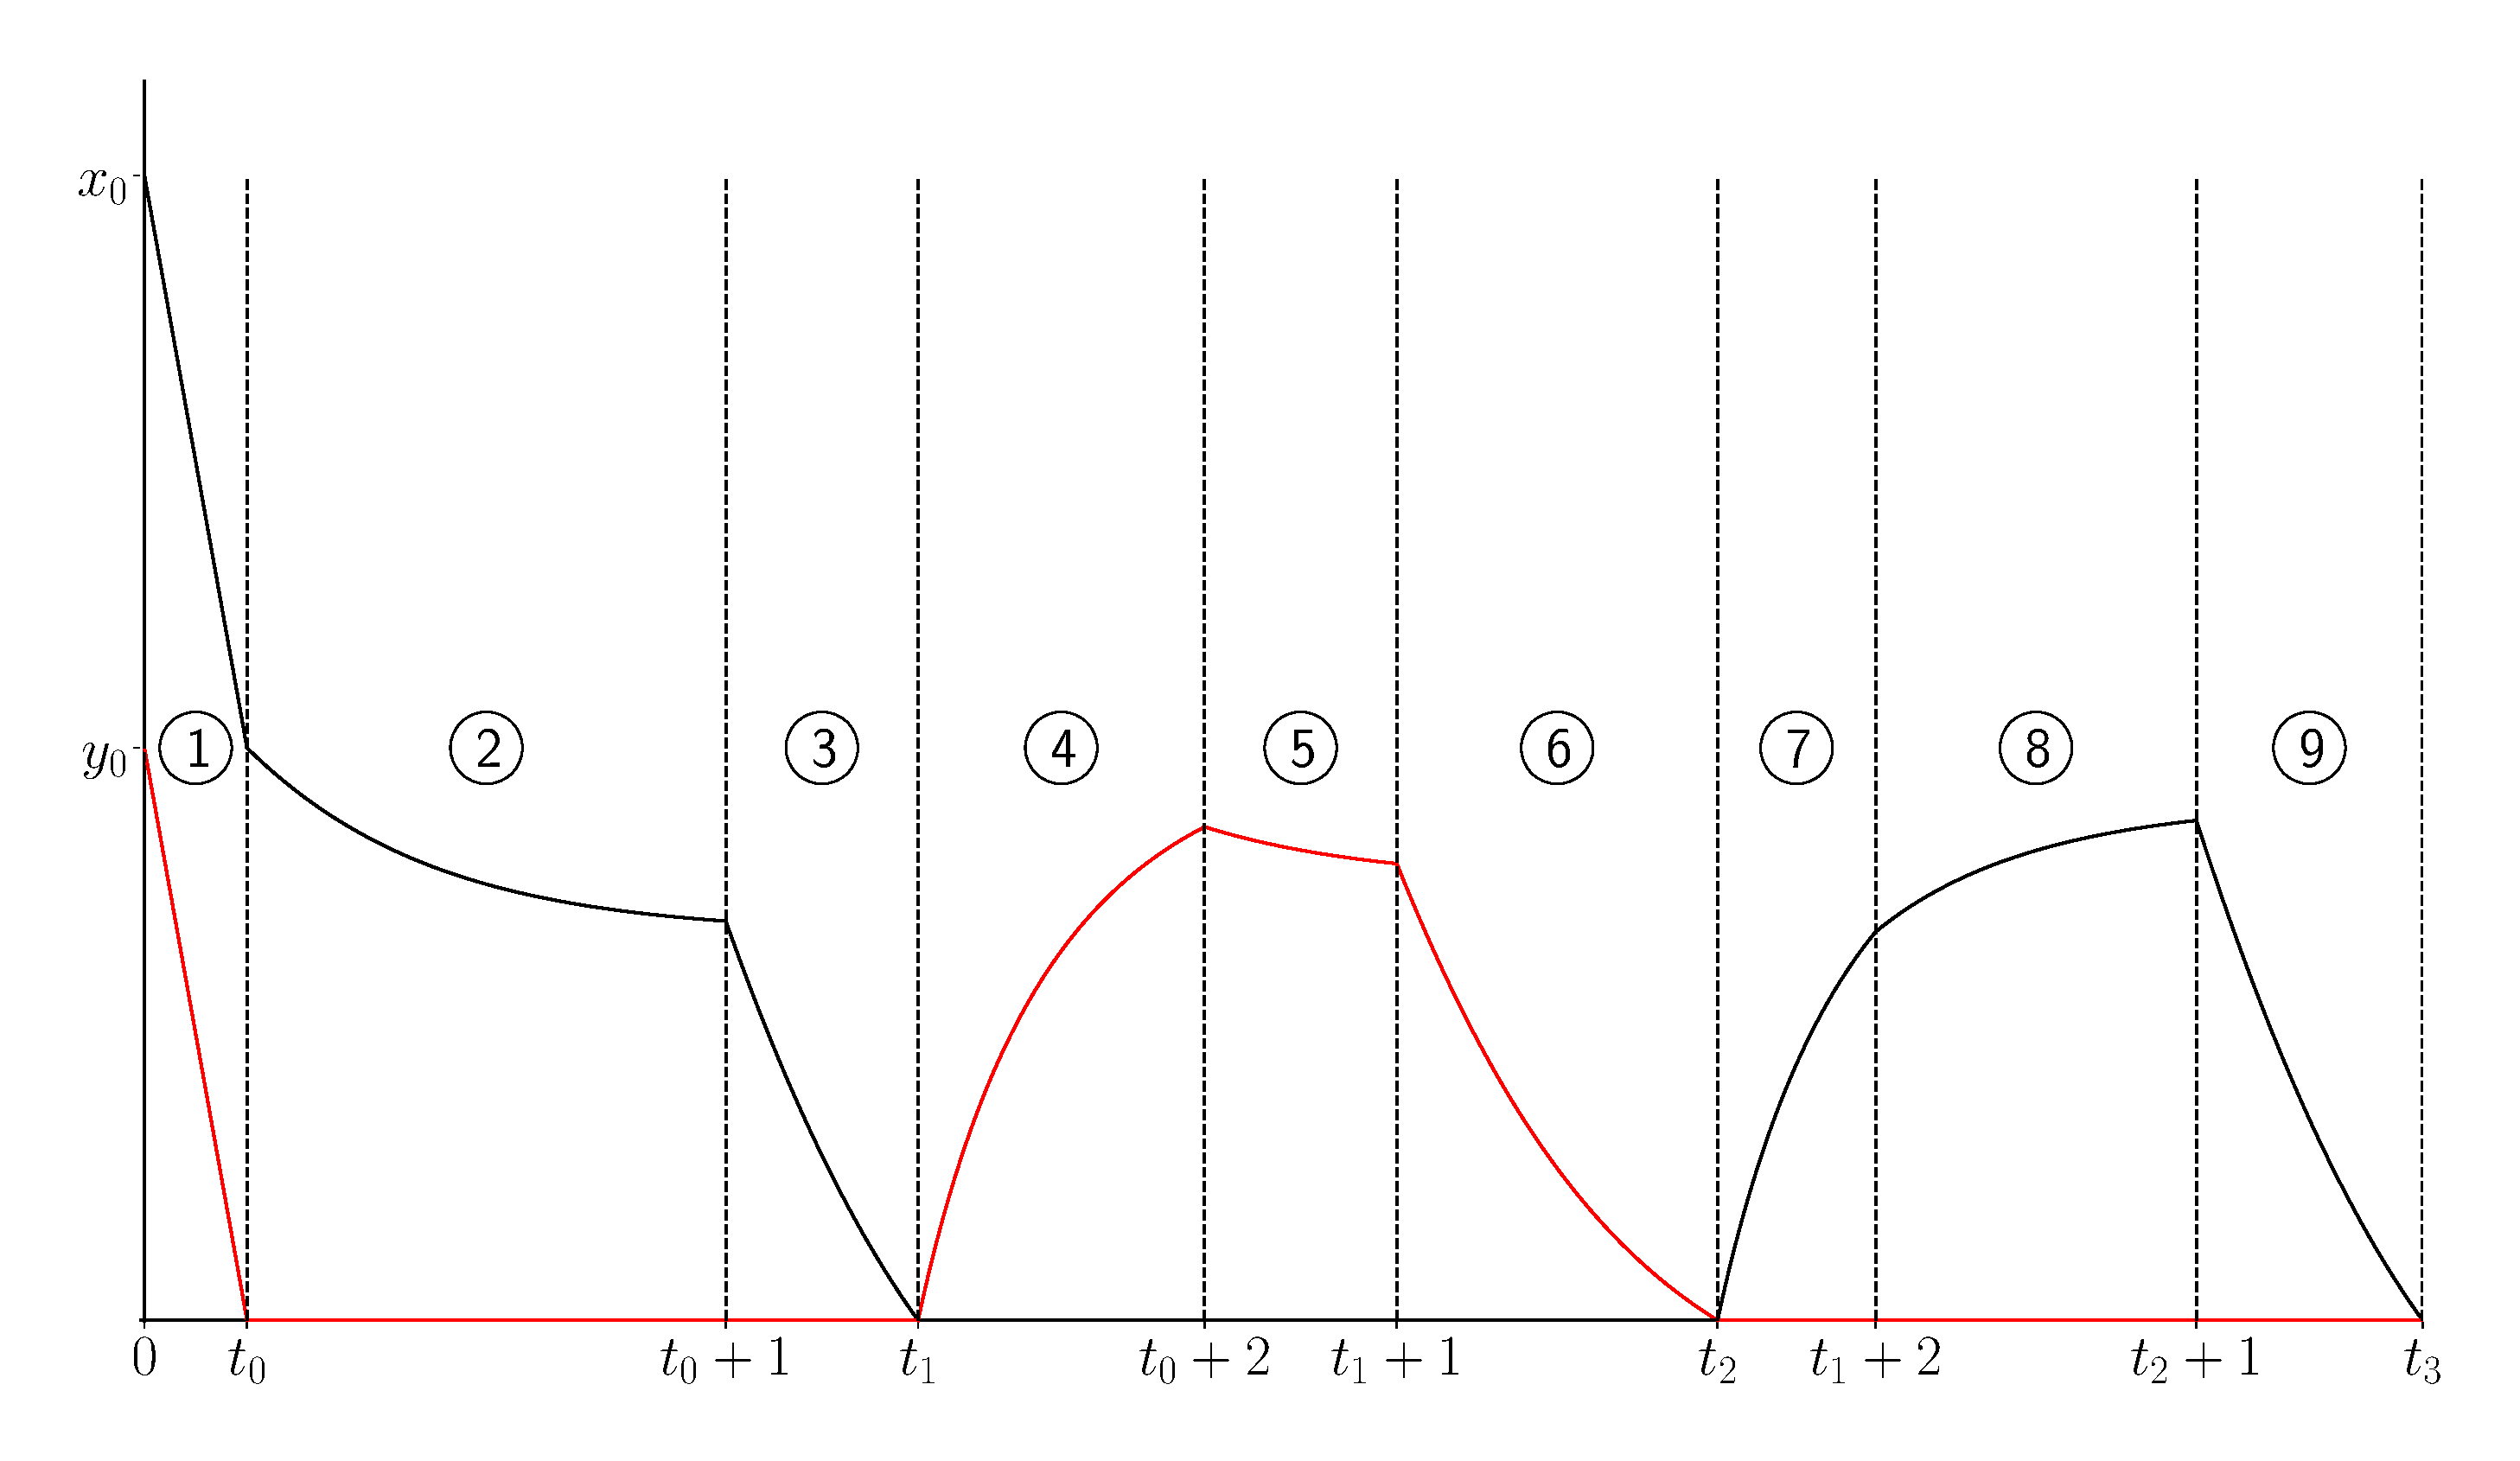
\includegraphics[width=\textwidth]{cluster_step_by_step.eps}
	\caption{Решение системы \eqref{eq:system_main_relay}, построенное методом шагов. Чёрная линия --- компонента решения $x$, красная линия --- компонента решения $y$. Числа в кругах означают номер шага построения.}
	\label{fig:cluster_step_by_step}
\end{figure}


\subsection{Метод шагов}
\paragraph{Шаг 1.} На отрезке $[0, t_0]$ система \eqref{eq:system_main_relay} принимает вид
%
\begin{equation}
	\label{eq:step1_system}
	\begin{cases}
		\dot{x} = -\beta,\\
		\dot{y} = -\beta.
	\end{cases}
\end{equation}

Она имеет решение \eqref{eq:step1_solution}, которое продолжается до точки $t_0 = \dfrac{y_0}{\beta}$, в которой $y(t_0) = 0$.

\paragraph{Шаг 2.} Рассмотрим следующий отрезок построения решения $[t_0, t_0 + 1]$. C учётом условия \eqref{eq:constraint_2}, при $y < 0$ второе уравнение системы \eqref{eq:system_main_relay} принимает вид
\[
\dot{y} = -\beta + \alpha \delta (n - 1) > 0,
\]
а при $y > 0$ получаем $\dot{y} = -\beta < 0$.

Следовательно, решение может быть продолжено только вдоль прямой $y = 0$ до момента, когда компонента $x$ также обратится в ноль. Иллюстрация динамики системы в точке $t= t_0$ приведена на рис. \ref{fig:dynamics_t0}. Система \eqref{eq:system_main_relay} принимает вид

\begin{equation}
	\label{eq:step2_system}
	\begin{cases}
		\dot{x} = -\beta + g_y(0, t) \alpha \delta n e^{-x},\\
		\dot{y} = -\beta + g_y(0, t) \alpha \delta (n - 1),
	\end{cases}
\end{equation}
%
Из второго уравнения и условия $\dot{y} = 0$ находим $g_y(0, t) = \frac{\beta}{\alpha \delta (n - 1)}$ при $t \in [t_0, t_0 + 1]$. Подставляя это значение в первое уравнение, получаем начальную задачу Коши
\begin{equation}
	\label{eq:step2_start}
	\dot{x} = -\beta + \beta\cdot\dfrac{n}{n - 1}e^{-x}, \quad x|_{t = t_0} = x_0 - \beta t_0.
\end{equation}

\begin{lemma}
	\label{lm:default_equation}
	Начальная задача Коши 
	\[
	\dot{x} = -\beta + \beta \theta e^{-x}, \quad x \vert_{t = t_*} = x_*,
	\]
	где $\theta, x_*, t_*$ --- вещественные константы, имеет при $t > t_*$ решение 
	\[
	x = x_* - \beta (t - t_*) + \ln\left(1 + \theta e^{-x_*} (e^{\beta(t - t_*)} - 1)\right) =
	-\beta t + \ln\left(e^{x_* + \beta t_*} + \theta (e^{\beta t} - e^{\beta t_*})\right).
	\]
	%\[
	%x = -\beta t + \ln\left(e^{x_* + \beta t_*} + \theta (e^{\beta t} - e^{\beta %t_*})\right).
	%\]
\end{lemma}

\begin{proof}
	После замены $x = z - \beta t$, $z_* = z \vert_{t = t_*} = x_* + \beta t_*$ получаем уравнение с разделяющимися переменными
	\[
	e^{z} \dot{z} = \beta \cdot \theta e^{\beta t}.
	\]
	Интегрируя, получаем
	\[
	\int\limits_{z_*}^z e^{\tilde{z}} \, d\tilde{z} = \int\limits_{t_*}^{t} \beta \theta e^{\beta \tilde{t}}\,d\tilde{t},
	\]
	\[
	e^z - e^{z_*} = \theta (e^{\beta t} - e^{\beta t_*}).
	\]
	После обратной замены и элементарных преобразований получаем требуемое.
\end{proof}

Применяя лемму \ref{lm:default_equation} к уравнению \eqref{eq:step2_start} с условиями $\theta = \dfrac{n}{n - 1}$, $t_* = t_0$, $x_* = x_0 - \beta t_0$, получаем решение \eqref{eq:step2_solution}. Решение продолжается либо до точки $t_0 + 1$, либо до точки, в которой $x = 0$. Докажем, что всегда реализуется первый случай.

\begin{lemma}
	\label{lm:solution_monotone}
	Пусть $A, B$ --- вещественные константы такие, что $A + B e^{\beta t} > 0$ при $t > 0$. Функция $f(t) = -\beta t + \ln\left(A + B e^{\beta t}\right)$ монотонна на всей области определения.
\end{lemma}
\begin{proof}
	Продифференцируем $f(t)$:
	\[
	f'(t) = -\beta + \beta \dfrac{B e^{\beta t}}{A + B e^{\beta t}} = -\dfrac{A \beta}{A + B e^{\beta t}}.
	\]
	Знаменатель по условию положителен, поэтому производная знакопостоянна и имеет тот же знак, что $-A \beta$. Следовательно, $f$ монотонна.
\end{proof}

По лемме \ref{lm:solution_monotone}, решение $x(t)$ на втором шаге монотонно. Чтобы убедиться, что оно положительно на отрезке $[t_0, t_0 + 1]$, достаточно проверить условие $x(t_0 + 1) > 0$.
%
\[
x(t_0 + 1) = x_0 - \beta (t_0 + 1) + \ln\left(1 + \frac{n}{n - 1}e^{-x_0 + \beta t_0} (e^{\beta} - 1)\right) > 0.
\]
%
После элементарных преобразований получаем неравенство
\[
e^{x_0 - \beta t_0} > \dfrac{n - e^\beta}{n - 1},
\]
которое верно, поскольку левая часть больше $1$, а правая --- меньше.

Следовательно, $x > 0$ на отрезке $[t_0, t_0 + 1]$.

\paragraph{Шаг 3.} На отрезке $[t_0 + 1, t_1]$ система \eqref{eq:system_main_relay} принимает вид
\begin{equation}
	\label{eq:system_step3}
	\begin{cases}
		\dot{x} = -\beta + \alpha \delta n e^{-x} g_y(0, t),\\
		\dot{y} = -\beta + \alpha \left(g_y(0, t - 1) + \delta (n - 1) g_y(0, t)\right).
	\end{cases}
\end{equation}

Учитывая условия $\dot{y} = 0$, $g_y(0, t - 1) = \frac{\beta}{\alpha \delta (n - 1)}$, из второго уравнения находим $g_y(0, t) = \frac{\beta}{\alpha} \cdot \frac{\delta(n - 1) - 1}{\delta^2 (n - 1)^2}$. Подставляя это значение в первое уравнение, получаем
\[
\dot{x} = -\beta + \beta \cdot \dfrac{n (\delta(n - 1) - 1)}{\delta (n - 1)^2} e^{-x} \quad \text{при } t\in[t_0 + 1, t_1].
\]
%
Применяя лемму \ref{lm:default_equation} при $\theta = \frac{n (\delta(n - 1) - 1)}{\delta (n - 1)^2}$, получаем решение \eqref{eq:step3_solution} при $i = 0$.

Аналитический вид решения сохраняется до точки $t_0 + 2$ или до точки $t_1$, в которой $x(t_1) = 0$. По лемме \ref{lm:solution_monotone}, $x(t)$ монотонна на третьем шаге. Следовательно, $t_1 \in (t_0 + 1, t_0 + 2)$ тогда и только тогда, когда $x(t_0 + 2) < 0$.

\begin{lemma}
	\label{lm:t1_one_step}
	Неравенство \eqref{eq:constraint_1} равносильно условию $t_1 \in (t_0 + 1, t_0 + 2)$.
\end{lemma}
\begin{proof}
	Подставим $t = t_0 + 1$ в \eqref{eq:step2_solution}:
	\begin{multline*}
		x(t_0 + 1) = x_0 - \beta (t_0 + 1) + \ln\left(1 + \frac{n}{n - 1} e^{-x_0 + \beta t_0}  (e^{\beta} - 1)\right) =\\= -\beta + \ln\left(e^{x_0 - y_0} + \dfrac{n}{n - 1}(e^{\beta} - 1)\right).
	\end{multline*}
	
	Подставим найденное значение $x(t_0 + 1)$ и $t = t_0 + 2$ в формулу \eqref{eq:step3_solution}:
	\small
	\begin{multline*}
		x(t_0 + 2) = -\beta (t_0 + 2) + \ln\left(e^{x(t_0 + 1) + \beta (t_0 + 1)} + \frac{n (\delta(n - 1) - 1)}{\delta (n - 1)^2} (e^{\beta (t_0 + 2)} - e^{\beta (t_0 + 1)})\right) = \\ = -2\beta + \ln\left(e^{x(t_0 + 1) + \beta} + \frac{n (\delta(n - 1) - 1)}{\delta (n - 1)^2} (e^{2\beta} - e^{\beta})\right) = \\ = -2\beta + \ln\left(e^{x_0 - y_0} + \dfrac{n}{n - 1}(e^{\beta} - 1) + \frac{n (\delta(n - 1) - 1)}{\delta (n - 1)^2} (e^{2\beta} - e^{\beta})\right).
	\end{multline*}
	\normalsize
	
	Неравенство $x(t_0 + 2) < 0$ эквивалентно \eqref{eq:constraint_1}, что можно проверить элементарными преобразованиями.
\end{proof}

\paragraph{Шаг 4.} На отрезке $[t_1, t_0 + 2]$ система \eqref{eq:system_main_relay} принимает вид
\small
\begin{equation}
	\begin{cases}
		\dot{x} = -\beta + \alpha \left(\delta (m - 1) g_x(x, t) + \delta n e^{y - x} g_y(y, t)\right)\\
		\dot{y} = -\beta + \alpha \left(e^{y(t - 1) - y} g_y(0, t - 1) + \delta m e^{x - y} g_x(x, t) + \delta (n - 1) g_y(y, t)\right).
	\end{cases}
\end{equation}
\normalsize
% Если $x < 0$, то из первого уравнения получаем $\dot{x} \geqslant -\beta + \alpha(m - 1) > 0$. По лемме \ref{lm:signed_solution}, $x \geq 0$. Если $x > 0$ в точке $\tau \in (t_1, t_0 + 2)$, то либо $y > 0$ и $\dot{x} = -\beta < 0$, либо $y = 0$ и система примет вид \eqref{eq:system_step3}, для которой также $\dot{x} < 0$. По лемме \ref{lm:signed_solution}, $x \leq 0$. Значит, на 4-м шаге $x \equiv 0$.

Если $x < 0$, то из первого уравнения получаем $\dot{x} \geqslant -\beta + \alpha \delta (m - 1) > 0$. Если $x > 0$ в точке $t \in (t_1, t_0 + 2)$, то либо $y > 0$ и $\dot{x} = -\beta < 0$, либо $y = 0$ и система примет вид \eqref{eq:system_step3}, для которой также $\dot{x} < 0$. Тогда решение может быть продолжено только вдоль прямой $x = 0$. Иллюстрация динамики системы в точке $t=t_1$ приведена на рис. \ref{fig:dynamics_t1}.

Система \eqref{eq:system_main_relay} примет вид
%
\begin{equation}
	\label{eq:step4_system}
	\begin{cases}
		\dot{x} = -\beta + \alpha \delta (m - 1) g_x(0, t),\\
		\dot{y} = -\beta + \alpha \left(e^{-y} g_y(0, t - 1) + \delta m e^{-y} g_x(0, t)\right).
	\end{cases}
\end{equation}
%
Из первого уравнения находим $g_x(0, t) = \frac{\beta}{\alpha \delta (m - 1)}$. С учётом $g_y(0, t - 1) = \frac{\beta}{\alpha \delta (n - 1)}$, второе уравнение примет вид
\[
\dot{y} = -\beta + \beta \left(\dfrac{1}{\delta(n - 1)} + \dfrac{m}{m - 1} \right) e^{-y}.
\]
%
Применяя лемму \ref{lm:default_equation} с условиями
\[
\theta = \dfrac{1}{\delta(n - 1)} + \dfrac{m}{m - 1}, \quad t_* = t_1, \quad y(t_*) = 0,
\]
получаем решение \eqref{eq:step4_solution} системы на отрезке $[t_1, t_0 + 2]$:

Легко проверить, что условие $y > 0$ для второго уравнения из \eqref{eq:step4_solution} эквивалентно верному неравенству
\[
\dfrac{1}{\delta(n - 1)} + \dfrac{m}{m - 1} > 1,
\]
поэтому новых точек переключения на отрезке $[t_1, t_0 + 2]$ не появляется.

\paragraph{Шаг 5.} На отрезке $[t_0 + 2, t_1 + 1]$ система имеет вид \eqref{eq:step4_system} с одним изменением: $g_y(0, t - 1) = \frac{\beta}{\alpha} \cdot \frac{\delta(n - 1) - 1}{\delta^2 (n - 1)^2}$.
%
Тогда на 5-м шаге система имеет решение \eqref{eq:step5_solution}.
%
Как и в прошлом случае, убедимся, что $y > 0$. Действительно, условие $y > 0$ для второго уравнения из \eqref{eq:step5_solution} эквивалентно
\[
\frac{\delta(n - 1) - 1}{\delta^2 (n - 1)^2} + \dfrac{m}{m - 1} > \dfrac{e^{\beta t} - e^{y(t_0 + 2) + \beta (t_0 + 2)}}{e^{\beta t} - e^{\beta (t_0 + 2)}},
\]
что верно, поскольку левая часть больше $1$, а правая --- меньше.

\paragraph{Шаг 6 и последующие шаги.} Поскольку $g_x(0, t) = \frac{\beta}{\alpha \delta (m - 1)}$ на промежутке $[t_1, t_1 + 1]$, следующая точка переключения --- либо $t_1 + 2$, либо $t_2 \in (t_1 + 1, t_1 + 2)$ при условии $y(t_2) = 0$. Предположим, что реализуется второй случай; соответствующие ограничения на параметры сформулируем и докажем позже.

Тогда при $t \in [t_1 + 1, t_2]$ система \eqref{eq:system_main_relay} имеет вид
%
\begin{equation}
	\label{eq:step6_system}
	\begin{cases}
		\dot{x} = -\beta + \alpha \left(\frac{\beta}{\alpha \delta (m - 1)} + \delta (m - 1) g_x(0, t)\right)\\
		\dot{y} = -\beta + \alpha \delta m e^{-y} g_x(0, t).
	\end{cases}
\end{equation}
%
Заметим, что она совпадает с системой \eqref{eq:system_step3} с точностью до замены $x$ на $y$, $m$ на $n$, $g_y$ на $g_x$ и начального значения $y(t_1 + 1)$. Значит, следующие шаги построения решения аналогичны шагам 3~--~5. Общий вид решения на отрезках $[t_1 + 1, t_2]$, $[t_2, t_1 + 2]$, $[t_1 + 2, t_2 + 1]$ приведён в формулах \eqref{eq:step6_solution}, \eqref{eq:step7_solution},  \eqref{eq:step8_solution}.

При условии, что компонента $x$ обращается в ноль в точке $t_3 \in (t_2 + 1, t_2 + 2)$, решение на отрезке $[t_2 + 1, t_3]$ описывается формулами \eqref{eq:step9_solution} для $i = 0$.

Построение решения на следующих шагах, соответствующих $i \geqslant 1$ в условии теоремы \ref{thm:relay_solution}, в точности повторяет шаги, начиная с 4-го.

\subsection{Ограничения на параметры системы}
Опишем достаточные условия на параметры, гарантирующие $t_{i + 1} \in (t_i + 1, t_i + 2)$ при $i \geqslant 1$.

Обозначим (см. рисунок \ref{fig:x_star})
\begin{equation}
	\label{eq:x_star_definition}
	x^*_i = x(t_{2i} + 1), \quad y^*_i = y(t_{2i - 1} + 1).
\end{equation}

\begin{figure}
	\centering
	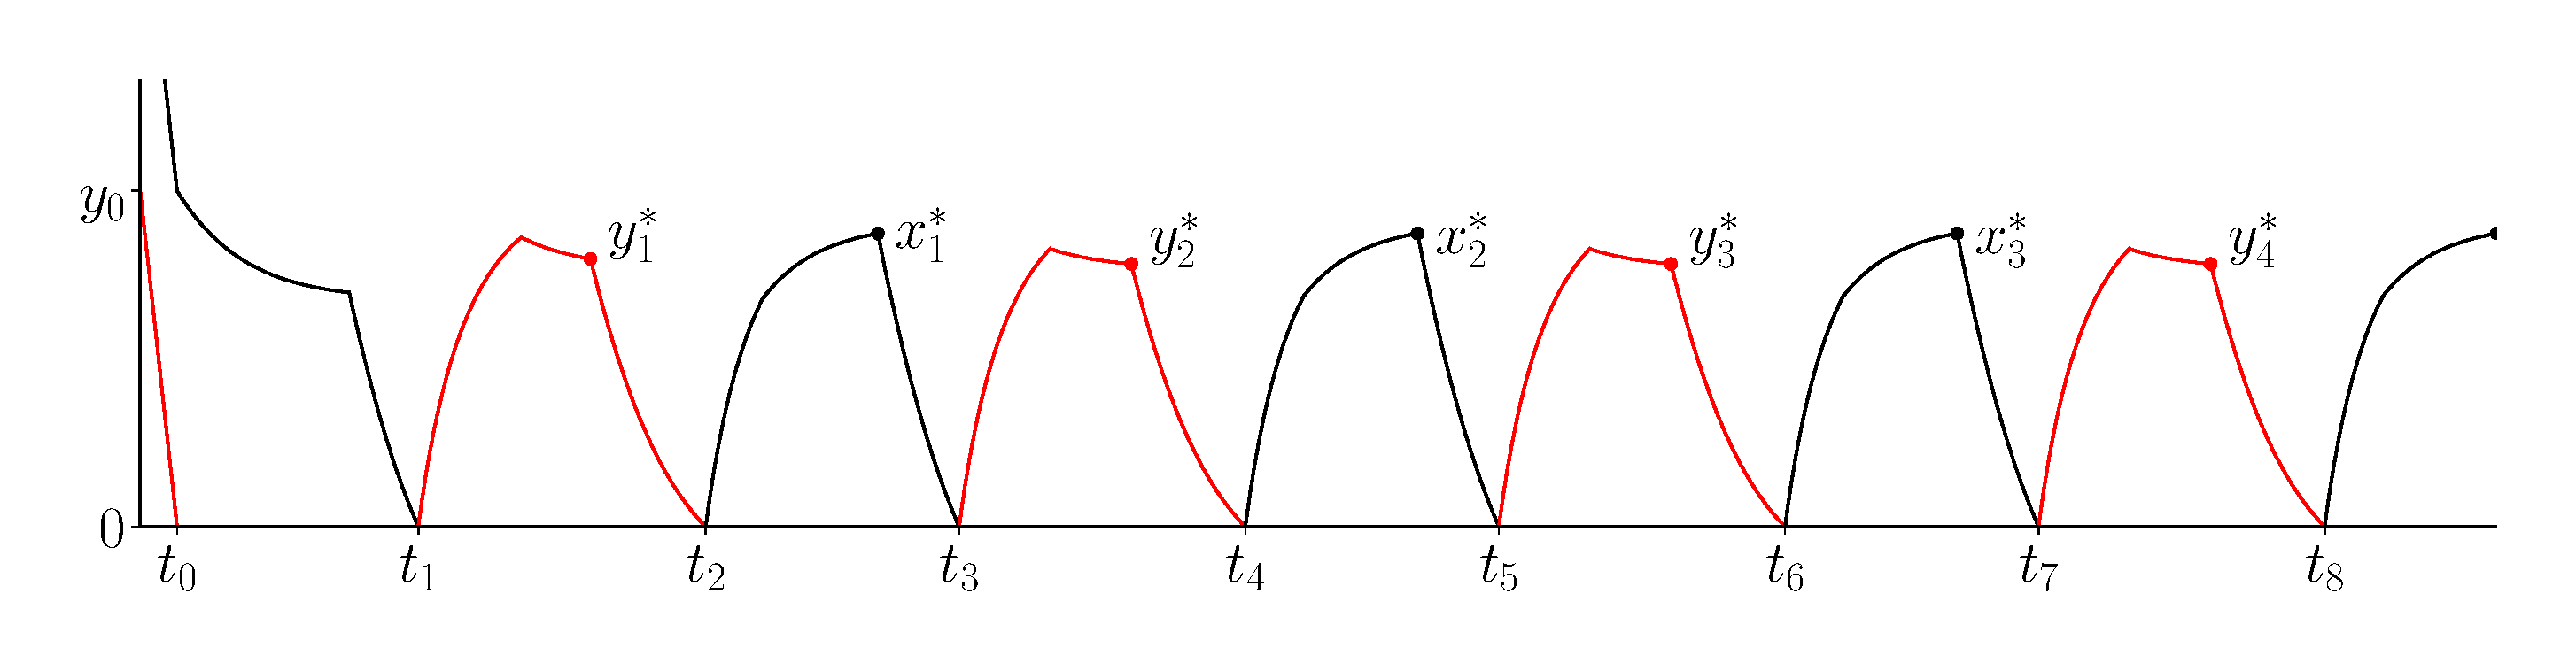
\includegraphics[width=\textwidth]{cluster_stars.eps}
	\caption{Последовательности значений $x^*_i$ и $y^*_i$, определённые формулами \eqref{eq:x_star_definition}. По каждому из значений решение системы \eqref{eq:system_main_relay} продолжается однозначно. В лемме \ref{lm:convergence_x_star} доказывается сходимость этих последовательностей.}
	\label{fig:x_star}
\end{figure}

\begin{figure}
	\begin{minipage}{0.48\textwidth}
		\centering
		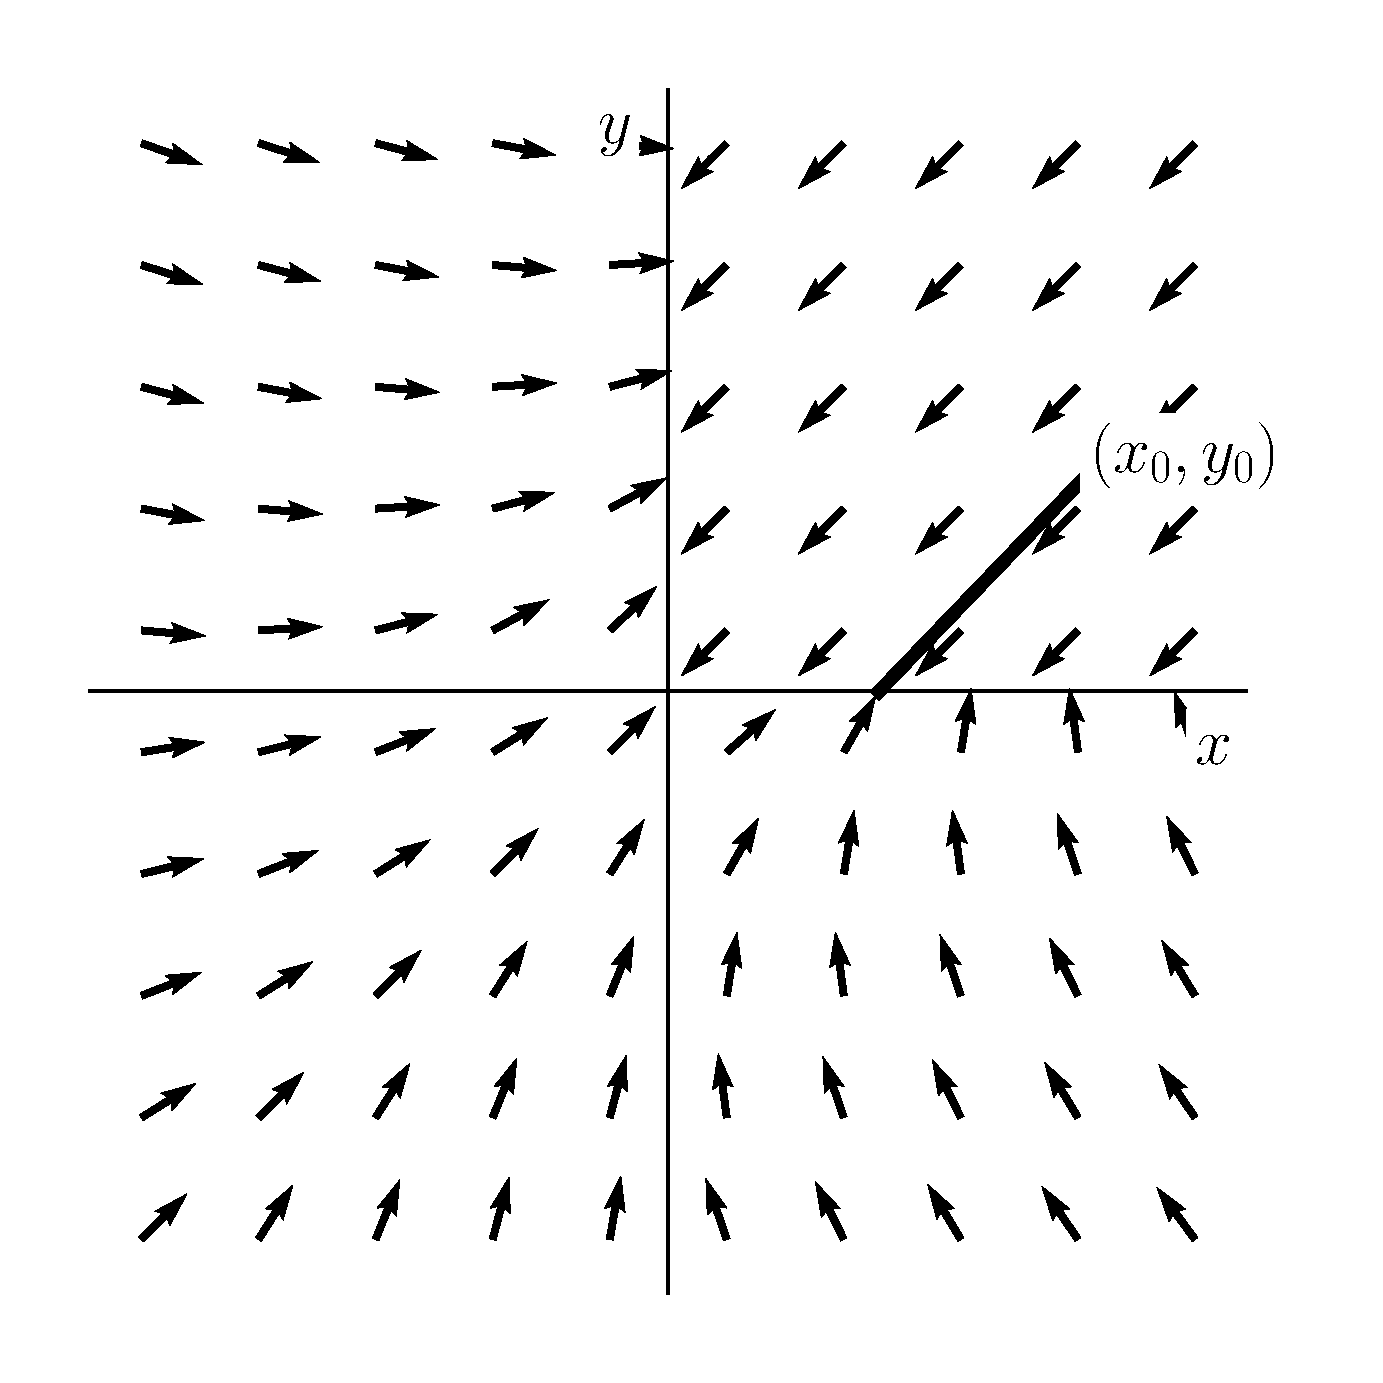
\includegraphics[width=\linewidth]{cluster_dynamics_t0.eps}
		\captionsetup{width=0.9\textwidth} 
		\caption{Векторное поле $(\dot{x}, \dot{y})$ в момент времени $t = t_0$. Жирной линией изображена проекция фазовой траектории на плоскость $(x, y)$ при $t \in [0, t_0]$. %Поскольку с обеих сторон прямой $y = 0$ векторы $(\dot{x}, \dot{y})$ направлены к ней, решение продолжается вдоль прямой.
		}
		\label{fig:dynamics_t0}
	\end{minipage}\hfill
	\begin{minipage}{0.48\textwidth}
		\centering
		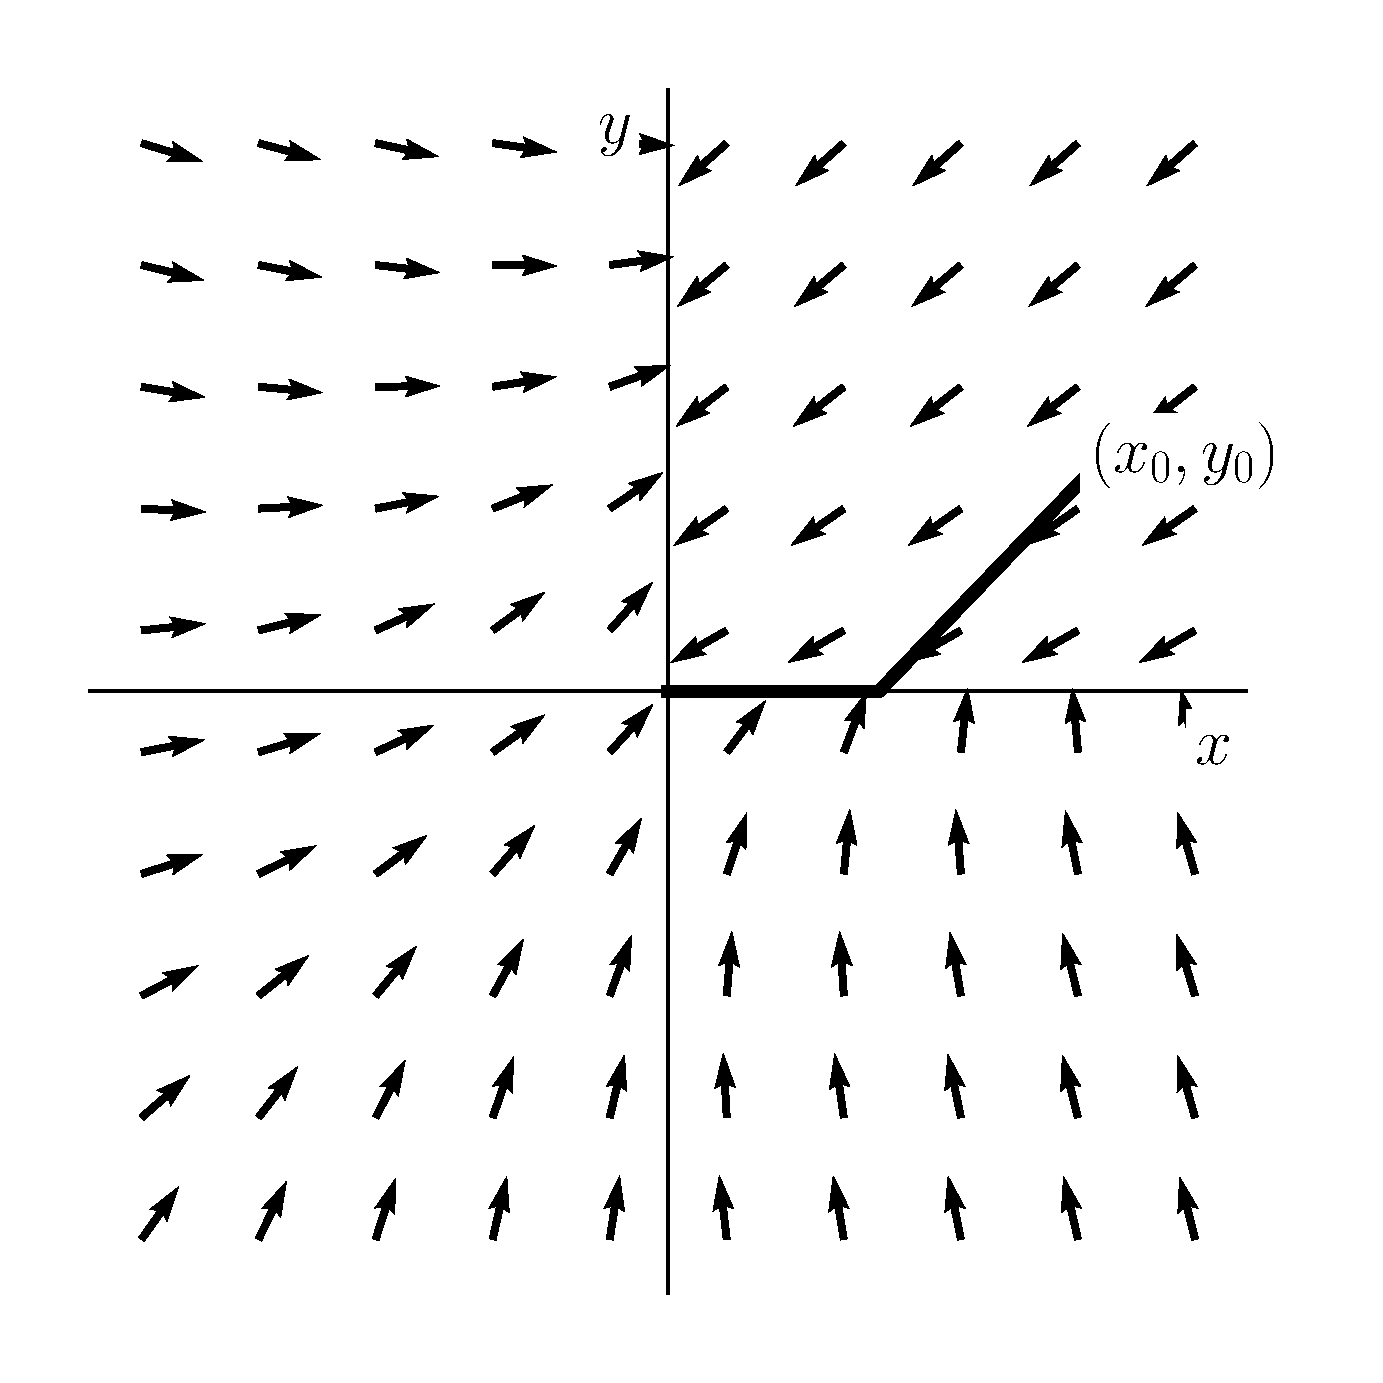
\includegraphics[width=\linewidth]{cluster_dynamics_t1.eps}
		\captionsetup{width=0.9\textwidth} 
		\caption{Векторное поле $(\dot{x}, \dot{y})$ в момент времени $t = t_1$. Жирной линией изображена проекция фазовой траектории на плоскость $(x, y)$ при $t \in [0, t_1]$.}
		\label{fig:dynamics_t1}
	\end{minipage}
\end{figure}

\begin{lemma}
	\label{lm:xy_star_bounds}
	При условии $t_{i + 1} \in (t_i + 1, t_i + 2)$ для любого $i \geqslant 1$ верны следующие оценки:
	\footnotesize
	\begin{multline}
		\label{eq:x_star_bound}
		-\beta + \ln\left(1 + \left( \frac{\delta(m - 1) - 1}{\delta^2 (m - 1)^2} + \dfrac{n}{n - 1} \right)(e^{\beta} - 1) \right) < x^*_i < \\ -\beta + \ln\left(1 + \left( \dfrac{1}{\delta(m - 1)} + \dfrac{n}{n - 1} \right)(e^{\beta} - 1) \right)
	\end{multline}
	\begin{multline}
		\label{eq:y_star_bound}
		-\beta + \ln\left(1 + \left( \frac{\delta(n - 1) - 1}{\delta^2 (n - 1)^2} + \dfrac{m}{m - 1} \right)(e^{\beta} - 1) \right) < y^*_i < \\ -\beta + \ln\left(1 + \left( \dfrac{1}{\delta(n - 1)} + \dfrac{m}{m - 1} \right)(e^{\beta} - 1) \right)
	\end{multline}
	\normalsize
\end{lemma}
\begin{proof}
	Рассмотрим отрезок $[t_2, t_2 + 1]$.
	
	На отрезке $[t_2, t_1 + 2]$ действуют формулы \eqref{eq:step7_solution}. Пусть $\tau = t - t_2$, тогда
	%
	\[
	x(t_2 + \tau) = - \beta \tau + \ln\left( 1 + \left(\dfrac{1}{\delta(m - 1)} + \dfrac{n}{n - 1}\right) (e^{\beta \tau} - 1) \right).
	\]
	Пусть $\tau^* = t_1 + 2 - t_2$, тогда
	\[
	x(t_1 + 2) = x(t_2 + \tau^*) = -\beta \tau^* + \ln\left( 1 + \left(\dfrac{1}{\delta(m - 1)} + \dfrac{n}{n - 1}\right) (e^{\beta \tau^*} - 1) \right).
	\]
	
	На отрезке $[t_1 + 2, t_2 + 1]$ действуют формулы \eqref{eq:step8_solution}. Подставим вычисленное значение $x^* = x(t_1 + 2)$ и вычислим $x^*_1 = x(t_2 + 1)$:
	%
	\begin{multline}
		\label{eq:tau_to_t2+1}
		x^*_1 = x(t_2 + 1) = -\beta + \ln\Bigg( 1 - \left(\frac{1}{\delta(m - 1)} + \frac{n}{n - 1}\right) + \\ + \left(\frac{n}{n - 1} + \frac{\delta(m - 1) - 1}{\delta^2 (m - 1)^2}\right) e^{\beta} + \left(\frac{1}{\delta(m - 1)} - \frac{\delta(m - 1) - 1}{\delta^2 (m - 1)^2}\right) e^{\beta \tau^*} \Bigg).
	\end{multline}
	%
	Рассмотрим 
	Заметим, что 
	\[
	\frac{1}{\delta(m - 1)} - \frac{\delta(m - 1) - 1}{\delta^2 (m - 1)^2} = \frac{1}{\delta^2 (m - 1)^2} > 0,
	\]
	поэтому функция \eqref{eq:tau_to_t2+1} возрастает по $\tau^* \in [0, 1]$, следовательно, 
	%
	\[
	x^*_1 \vert_{\tau^* = 0} < x^*_1 < x^*_1 \vert_{\tau^* = 1}
	\]
	Вычисляя явно, получаем оценки \eqref{eq:x_star_bound} для $x_1^*$. Оценки \eqref{eq:x_star_bound} и \eqref{eq:y_star_bound} для $x_i^*$ и $y_i^*$ получаются аналогично. 
	
\end{proof}

\begin{lemma}
	\label{lm:constraints_all}
	Пусть верны ограничения \eqref{eq:constraint_1}, \eqref{eq:constraint_2}, \eqref{eq:constraint_3}. Тогда $t_{i + 1} \in (t_i + 1, t_i + 2)$ при любом целом $i \geqslant 0$.
\end{lemma}
\begin{proof}
	
	База индукции $t_1 \in (t_0 + 1, t_0 + 2)$ доказана в лемме \eqref{lm:t1_one_step}. Индукция заключается в последовательной проверке условий $y(t_{2i - 1} + 2) < 0$ на шестом шаге в формуле \eqref{eq:step6_solution} и $x(t_{2i} + 2) < 0$ на девятом шаге в формуле~\eqref{eq:step9_solution} при любом $i \geqslant 1$.
	
	Не ограничивая общности, рассмотрим условие $y(t_1 + 2) < 0$. Из формул \eqref{eq:step6_solution} получаем:
	\[
	y(t_1 + 2) = -\beta + \ln\left(e^{y_1^*} + \frac{m(\delta(m - 1) - 1)}{\delta (m - 1)^2}(e^\beta - 1) \right).
	\]
	Поскольку справедлива оценка сверху из \eqref{eq:y_star_bound}, для выполнения $y(t_1 + 2) < 0$ достаточно
	%
	\small
	\[
	-\beta + \ln\Bigg(e^{-\beta} \left(1 + \left( \dfrac{1}{\delta(n - 1)} + \dfrac{m}{m - 1} \right)(e^{\beta} - 1)\right) + \frac{m(\delta(m - 1) - 1)}{\delta (m - 1)^2} (e^\beta - 1) \Bigg) < 0.
	\]
	\normalsize
	%
	Элементарными преобразованиями получаем второе неравенство \eqref{eq:constraint_3} для $y_1^*$. Аналогично, неравенство $x(t_2 + 2) < 0$ следует из первого неравенства \eqref{eq:constraint_3}, далее по индукции.
\end{proof}

\subsection{Доказательство теоремы \ref{thm:relay_solution}} 
Методом шагов были получены формулы \eqref{eq:step1_solution} -- \eqref{eq:step9_solution} в предположении $t_{i + 1} \in (t_i + 1, t_i + 2)$ при любом $i \geqslant 0$. В лемме \ref{lm:constraints_all} доказано, что справедливость этого предположения следует из ограничений \eqref{eq:constraint_1} и \eqref{eq:constraint_3}, поэтому теорема \ref{thm:relay_solution} доказана.


%%%%%%%%%%%%%%%%%%%%%%%%%%%%%%%%%%%%%%%%%%%
\section{Существование периодического решения}\label{sec:ch3/sect4}
%%%%%%%%%%%%%%%%%%%%%%%%%%%%%%%%%%%%%%%%%%%

\begin{lemma}
	\label{lm:convergence_x_star}
	Пусть выполнены условия теоремы \ref{thm:relay_solution}. Тогда последовательности $x^*_i$ и $y^*_i$, определённые формулами \eqref{eq:x_star_definition}, сходятся.
\end{lemma}
\begin{proof}
	
	Рассмотрим последовательность $x^*_i$. Докажем, что она ограничена и монотонна для достаточно больших $i$.
	
	Определим функцию $\Phi$ следующим образом. Рассмотрим систему \eqref{eq:system_main_relay} с~начальными условиями
	\begin{equation}
		\label{eq:lm_star_sonvergence_initial_problem}
	\begin{cases}
		x(t^*) = x^*,\\
		x(t) > 0 \quad \text{при } t \in [t^* - 1, t^*],\\
		y(t) = 0 \quad \text{при } t \in [t^* - 1, t^*],\\
		g_y(0, t) = \frac{\beta}{\alpha\delta(n - 1)} \quad \text{при } t \in [t^* - 1, t^*],
	\end{cases}
	\end{equation}
	где значение $x^*$ удовлетворяет ограничениям \eqref{eq:x_star_bound}, в которые вместо $x_i^*$ следует подставить $x^*$. Решение этой задачи соответствует решению релейной системы \eqref{eq:system_main_relay}, приведённому в теореме \ref{thm:relay_solution}, начиная с шага 9, см. формулу \eqref{eq:step9_solution}. Продолжим решение аналогично шагам 9, 4 -- 8, см. формулы \eqref{eq:step9_solution}, \eqref{eq:step4_solution} --- \eqref{eq:step8_solution}. В конце последнего шага решение приходит в точку $x = x^{**}, y = 0$. По~определению, полагаем $\Phi(x^*) = x^{**}$. Поскольку решение продолжается однозначно, такое определение функции $\Phi$ корректно.
	
	Из приведённого определения следует, что при всех $i \geq 0$ выполнено равенство
	\begin{equation}
		\label{eq:flow_relay}
		\Phi(x^*_i) = x^*_{i + 1}.
	\end{equation}
	
	Докажем, что $\Phi$ возрастает. Разложим его в композицию функций
	\[
	\Phi = \Phi_{tx} \circ \Phi_{yt} \circ \Phi_{ty} \circ \Phi_{xt}.
	\]
	Здесь функция $\Phi_{xt}$ сопоставляет значению $x^*$ момент времени $t^*_x$ в который компонента $x$ обращается в ноль. Решение на промежутке $[t^*, t_x^*]$ определяется аналогично шагу 9, см. формулу \eqref{eq:step9_solution}. Функция $\Phi_{ty}$ сопоставляет моменту времени $t^*_x$ значение $y^* = y(t^*_x + 1)$, решение на промежутке $[t_x^*, t_x^* + 1]$ определяется аналогично шагам 4 и 5, см. формулы \eqref{eq:step4_solution}, \eqref{eq:step5_solution}. Функции $\Phi_{yt}$ и $\Phi_{tx}$ определяются аналогично, здесь компоненты системы $x$ и $y$ меняются ролями.
	
	Тогда
	\begin{equation}
		x^*_i \underset{\Phi_{xt}}{\longmapsto} t_{2i + 1} \underset{\Phi_{ty}}{\longmapsto} y^*_{i + 1}  \underset{\Phi_{yt}}{\longmapsto}  t_{2i + 2} \underset{\Phi_{tx}}{\longmapsto}  x^*_{i + 1}.
	\end{equation}
	%Здесь каждое предыдущее значение в цепочке определяет последующее.
	
%	Отображения $x^*_i \mapsto t_{2i + 1}$ и $y^*_{i + 1} \mapsto t_{2i + 2}$ возрастают из условия непересечения интегральных кривых на каждом шаге решения.
	
	Отображения $\Phi_{xt}$ и $\Phi_{yt}$ возрастают из условия непересечения интегральных кривых на каждом шаге решения.
	
%	Пусть $\tau^* = t_{2i} + 2 - t_{2i + 1} $. Поскольку $t_{2i + 1} \in (t_{2i} + 1, t_{2i} + 2)$, $\tau^* \in (0, 1)$. Значение $y^*_{i + 1}$ выражается через $\tau^*$ аналогично \eqref{eq:tau_to_t2+1}
	Пусть $\tau^* = t_x^* - t^*$, $\tau^* \in (0, 1)$. Значение $x^*_t$ выражается через $\tau^*$ аналогично \eqref{eq:tau_to_t2+1}
%	\footnotesize
%	\[
%	y^*_{i + 1} = -\beta + \ln\Bigg( 1 - \left(\frac{1}{\delta(n - 1)} + \frac{m}{m - 1}\right) +  e^{\beta} \left(\frac{m}{m - 1} + \frac{\delta(n - 1) - 1}{\delta^2 (n - 1)^2}\right) +  \frac{e^{\beta \tau^*}}{\delta^2 (n - 1)^2} \Bigg).
%	\]
%	\normalsize
	\footnotesize
	\[
	x^*_t = -\beta + \ln\Bigg( 1 - \left(\frac{1}{\delta(m - 1)} + \frac{n}{n - 1}\right) +  e^{\beta} \left(\frac{n}{n - 1} + \frac{\delta(m - 1) - 1}{\delta^2 (m - 1)^2}\right) +  \frac{e^{\beta \tau^*}}{\delta^2 (m - 1)^2} \Bigg).
	\]
	\normalsize
	
%	Поскольку коэффициент $\frac{1}{\delta^2 (n - 1)^2}$ при $e^{\beta \tau^*}$ положителен, $y^*_{i + 1}$ возрастает по переменной $\tau^*$, соответственно, отображение $t_{2i + 1} \mapsto y^*_{i + 1}$ убывает.
	
	Поскольку коэффициент $\frac{1}{\delta^2 (m - 1)^2}$ при $e^{\beta \tau^*}$ положителен, $x^*_t$ возрастает по переменной $\tau^*$, соответственно, отображение $\Phi_{tx}$ убывает.
	
%	Аналогично, убывает отображение $t_{2i + 2} \mapsto x^*_{i + 1}$. Следовательно, $\Phi$ возрастает как композиция двух возрастающих и двух убывающих отображений.
	
	Аналогично, убывает отображение $\Phi_{ty}$. Следовательно, $\Phi$ возрастает как композиция двух возрастающих и двух убывающих отображений.
	
	Пусть $x^*_2 > x^*_1$. Тогда по индукции
	\[
	x^*_{i} > x^*_{i - 1} \Rightarrow \Phi(x^*_i) > \Phi(x^*_{i - 1}), \text{ т.~е. } x^*_{i + 1} > x^*_{i},
	\]
	следовательно, $x^*_i$ возрастает. Аналогично, если $x^*_2 < x^*_1$, то $x^*_i$ убывает, а если $x^*_2 = x^*_1$, то $x^*_i = x^*_1$ при любом $i$. Ограниченность $x^*_i$ следует из леммы \ref{lm:xy_star_bounds}. Следовательно, $x^*_i$ сходится. Аналогично, сходится последовательность $y^*_i$.
\end{proof}

\begin{figure}
	\centering
	\includegraphics[width=\textwidth]{star_map.eps}
	\caption{Иллюстрация к доказательству леммы \ref{lm:convergence_x_star}. На графике изображено решение начальной задачи Коши для системы \eqref{eq:system_main_relay} с~начальными условиями \eqref{eq:lm_star_sonvergence_initial_problem}.}
\end{figure}

\begin{theorem}
	\label{thm:periodic_relay_existence}
	При ограничениях \eqref{eq:constraint_1}, \eqref{eq:constraint_2}, \eqref{eq:constraint_3} система \eqref{eq:system_main_relay} имеет периодическое решение, описываемое на периоде $[t_1, t_3]$ формулами \eqref{eq:step4_solution} -- \eqref{eq:step9_solution}.
\end{theorem}
\begin{proof}
	Рассмотрим последовательность $x^*_i$. По лемме \ref{lm:convergence_x_star} она сходится, пусть $x^*_i \to \hat{x}$ при $i \to +\infty$. По построению, отображение $\Phi$ из леммы \ref{lm:convergence_x_star} непрерывно, поэтому
	\[
	x^*_{i + 1} = \Phi(x^*_i) \Rightarrow \hat{x} = \Phi(\hat{x}).
	\]
	Поскольку значение $x^*_1 = x(t_2 + 1)$ однозначно определяет решение при $t > t_2 + 1$, положив $x^*_1 = \hat{x}$, получим периодическое решение, описываемое на периоде формулами \eqref{eq:step4_solution} -- \eqref{eq:step9_solution}.
\end{proof}

%%%%%%%%%%%%%%%%%%%%%%%%%%%%%%%%%%%%%%%%%%%
\section{Результаты численного моделирования}\label{sec:ch3/sect5}
%%%%%%%%%%%%%%%%%%%%%%%%%%%%%%%%%%%%%%%%%%%

На рисунке \ref{fig:cluster_solution} приведены решения релейной системы \eqref{eq:system_main_relay} в сравнении с решениями соответствующих систем при различных $\gamma$. Численный эксперимент показал, что решение релейной системы \eqref{eq:system_main_relay} стремится к соответствующему решению системы \eqref{eq:system_main} при $\gamma \to +\infty$.

На рисунке \ref{fig:cluster_solution2} приведены решения релейной системы \eqref{eq:system_main_relay} для значений параметров, не удовлетворяющих условию \eqref{eq:constraint_3} (сверху) или условию \eqref{eq:constraint_2} (снизу). В обоих случаях, решение оказывается близко к периодическому.

%На рисунке \ref{fig:cluster_solution} приведено решение релейной системы \eqref{eq:system_main_relay} в сравнение с решением соответствующей системы при различных $\gamma$. Численный эксперимент показал, что решение релейной системы \ref{eq:system_main_relay} стремится к соответствующему решению системы \eqref{eq:system_main} при $\gamma \to +\infty$.

На рисунке \ref{fig:phase_portrait} приведён портрет системы \eqref{eq:system_main_relay} при различных значениях $\gamma$ в псевдофазовом пространстве (в координатах $x, y$). При $\gamma \to +\infty$ портрет вырождается в пару отрезков.

\begin{figure}[!htb]
	\centering
	
	\includegraphics[width=0.9\linewidth]{cluster_solution_1.eps}
	
	\smallskip
	
	\includegraphics[width=0.9\linewidth]{cluster_solution_2.eps}
	
	\caption{Решения системы \eqref{eq:system_main} для значений параметров $\alpha = 5.0$, $\beta = 3.7$, $m = 3$, $n = 4$, $\delta = 1.2$  (сверху); $\alpha = 3.0$, $\beta = 2.1$, $m = 2$, $n = 2$, $\delta = 1.5$ (снизу). Сплошными линиями изображены решения релейной системы \eqref{eq:system_main_relay}, штриховыми линиями --- решения системы при $\gamma = 200$, штрих-пунктирными линиями --- решения при $\gamma = 20$.
	}
	\label{fig:cluster_solution}
\end{figure}

\begin{figure}[!htb]
	\centering
	\includegraphics[width=0.9\linewidth]{cluster_solution_3.eps}
	
	\smallskip
	
	\includegraphics[width=0.9\linewidth]{cluster_solution_4.eps}
	
	\caption{Решения системы \eqref{eq:system_main} для значений параметров $\alpha = 10.0$, $\beta = 1.0$, $m = 5$, $n = 4$, $\delta = 1.02$, $\gamma = 500$ (сверху); $\alpha = 6.0$, $\beta = 1.6$, $m = 4$, $n = 3$, $\delta = 1.1$, $\gamma = 100$ (снизу).}
	\label{fig:cluster_solution2}
\end{figure}

\begin{figure}[!htb]
	\centering
	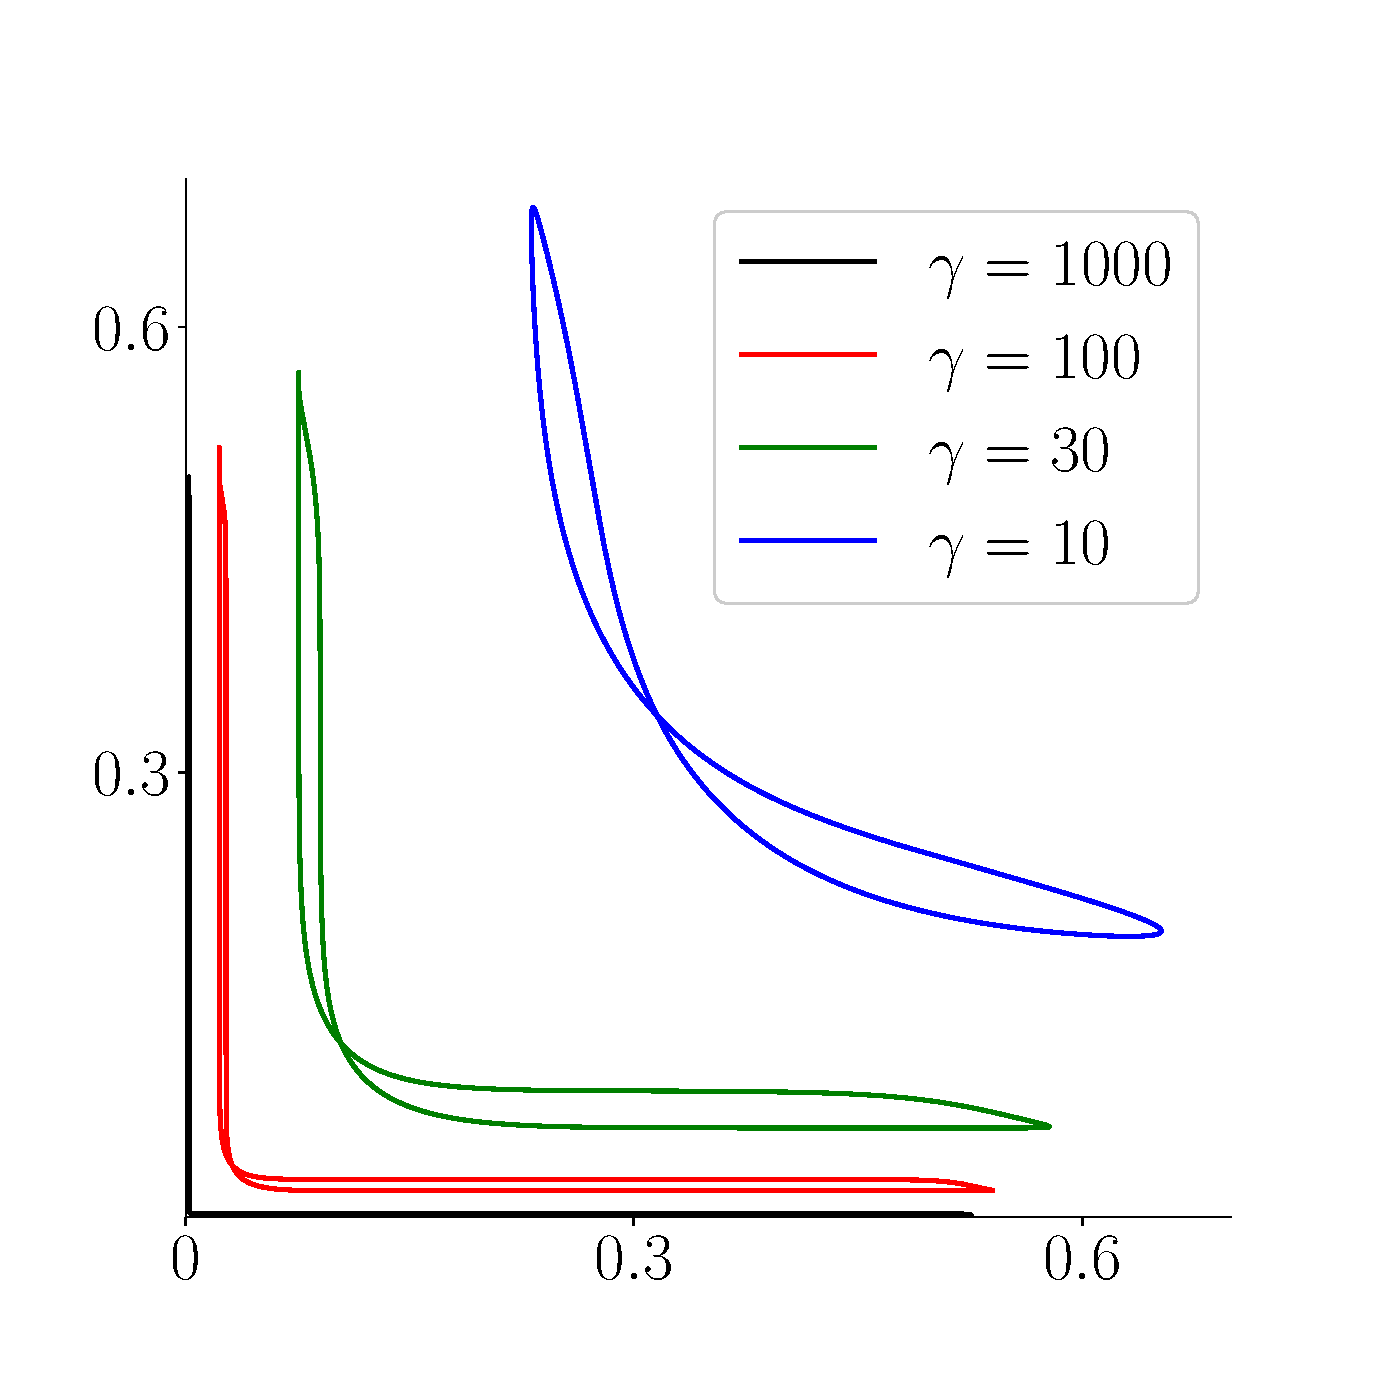
\includegraphics[width=0.5\linewidth]{cluster_phase_portrait.eps}
	\caption{Псевдофазовый портрет периодического решения системы \eqref{eq:system_main} при различных значениях $\gamma$. При $\gamma \gg 1$ портрет <<прижимается>> к координатным осям.}
	\label{fig:phase_portrait}
\end{figure} 

%%%%%%%%%%%%%%%%%%%%%%%%%%%%%%%%%%%%%%%%%%%
\section{Выводы к главе 3}\label{sec:ch3/sect6}
%%%%%%%%%%%%%%%%%%%%%%%%%%%%%%%%%%%%%%%%%%%
В данной главе было показано существование периодических режимов с кластерной синхронизацией в релейной системе осцилляторов Мэки-Гласса, а также дано их аналитическое описание.

Отметим, что возможно рассмотрение более общего случая: можно опустить требование $t_{i + 1} \in (t_{i} + 1, t_{i} + 2)$, при этом аналитический вид решения также представляется явно. Численное моделирование показывает существование периодических режимов в этом случае, однако доказательство его существования аналогично лемме \ref{lm:convergence_x_star} не обобщается ввиду немонотонности отображения $\Phi$. Также возможно построение решения с другими начальными условиями и ограничениями на параметры.
